\documentclass[aspectratio=169]{beamer}


%%%%%%%%%%%%%%%%%%%%%%%%%%%%%%%%%%%%%%%%%%%%%%%%%%%%%%%%%%%%%%%%%%%%%%%%%%%%%%%%%
% PREAMBLE

% DEFINE VARIABLES
\newcommand{\Lesson}{TEMA EJEMPLO}
\newcommand{\Subject}{Ejemplos, ejemplos, y ejemplos}
\newcommand{\Program}{Inversiones Financieras}
\newcommand{\Professor}{CUNEF Universidad}

% FOOTER WITH LOGO
\setbeamertemplate{footline}{
\hfill
\includegraphics[width=1.2cm]{figs/logo.png}\hspace{13cm}\vspace*{0.5cm}
\insertframenumber \hspace{1cm}
}

% FOOTER WITHOUT LOGO
\newcommand{\NoLogoFootline}{
    \setbeamertemplate{footline}{
    \hfill\vspace*{0.5cm}    
    }
}

% PACKAGES
\usepackage{framed, color}
\definecolor{shadecolor}{rgb}{1,0.9,0.8}
\usepackage[absolute,overlay]{textpos}
\usepackage{graphicx, tikz,xcolor}
\usepackage{multirow, bigstrut,epstopdf}
\usepackage{amsmath,relsize,bigdelim}
\usepackage{hyperref}
\hypersetup{
    colorlinks=true,
    linkcolor=blue,
    filecolor=magenta,      
    urlcolor=cyan,
}
\usepackage[font=tiny]{caption}

\setbeamercolor{block body}{bg=CUNEFGray!20,fg=Front}
\setbeamercolor{block title}{bg=CUNEFOrange,fg=white}

\usetikzlibrary{shapes.geometric, arrows.meta}


% IDENTATION OPTIONS
\setlength{\leftmargini}{1em} % for itemize and enumerate level 1
\setlength{\leftmarginii}{1em} % for itemize and enumerate level 2
\setlength{\leftmarginiii}{1em} % for itemize and enumerate level 3

% COLOR OPTIONS
\definecolor{CUNEFOrange}{RGB}{255, 87, 0}
\definecolor{CUNEFGray}{RGB}{214, 209, 196}
\definecolor{Front}{RGB}{21,31,108}
% BEAMER OPTIONS
\setbeamertemplate{navigation symbols}{}
\setbeamercolor{itemize item}{fg = CUNEFOrange}
\setbeamercolor{itemize subitem}{fg = CUNEFOrange}
\setbeamercolor{itemize subsubitem}{fg = CUNEFOrange}		
\setbeamercolor{enumerate item}{fg = CUNEFOrange}
\setbeamercolor{enumerate subitem}{fg = CUNEFOrange}
\setbeamercolor{enumerate subsubitem}{fg = CUNEFOrange}		
\setbeamercolor{normal text}{fg=Front}

\setbeamercolor{frametitle}{fg=CUNEFOrange}

% NEW TITLE SLIDE
\newcommand{\CUNEFTitleSlide}{\begin{frame}



%\begin{textblock*}{0.1\paperwidth}(0.01\paperwidth,0.01\paperwidth)
%\includegraphics[width=0.3\paperwidth]{Logo_WQU.png}
%\end{textblock*}

\vspace{2em}
%\centering\scriptsize{{\textcolor{CUNEFOrange}{\Lesson}}} \\[1em]
\centering\textbf{{\large\textcolor{CUNEFOrange}{Econometrics 2024/2025}}} \\ [1em]
\centering{\large\textcolor{CUNEFOrange}{}} \\ [1em]
\vspace{0.5em}
\centering{\normalsize\textcolor{CUNEFOrange}{Topic 2: Multiple Regression Analysis: Estimation}}
\end{frame}}

% NEW SLIDE TEMPLATE
\newcommand{\slide}[2]{\begin{frame}
%\begin{textblock*}{0.1\paperwidth}(0.01\paperwidth,0.01\paperwidth)
%\includegraphics[width=0.15\paperwidth]{Logo_WQU.png}
%\end{textblock*}


\begin{textblock*}{0.87\paperwidth}(0.05\paperwidth,1.2cm)
{\Large\textcolor{CUNEFOrange}{#1}}
\end{textblock*}

\begin{textblock*}{0.87\paperwidth}(0.05\paperwidth,2cm)
#2
\end{textblock*}

\begin{textblock*}{\paperwidth}(0.01\paperwidth,0.95\paperheight)
\noindent\begin{tikzpicture}
%\draw[CUNEFOrange] (0,0) rectangle (0.9\paperwidth,0.8em);
%\draw[CUNEFOrange] (0.9\paperwidth+0.01\paperwidth,0) rectangle (\paperwidth-0.02\paperwidth,0.8em);
%\node[right] at (0,0.4em) {\tiny\textcolor{CUNEFGray}{\Subject\enspace-- \Program\enspace-- \Professor\enspace}};
\end{tikzpicture}
{\tiny\textcolor{CUNEFGray}\thepage}
\end{textblock*}
\end{frame}
}
%%%%%%%%%%%%%%%%%%%%%%%%%%%%%%%%%%%%%%%%%%%%%%%%%%%%%%%%%%%%%%%%%%%%%%%%%%%%%%%%%

% TOC AT BEGINNING OF EACH SECTION
\AtBeginSection[]{
    \begin{frame}<beamer>
    \frametitle{\textcolor{CUNEFOrange}{Outline}}
    \tableofcontents[currentsection]
    \end{frame}
}



\begin{document}

%%%%%%%%%%%%%%%%%%%%%
% Title Page
%%%%%%%%%%%%%%%%%%%%
\NoLogoFootline
{\usebackgroundtemplate{%
  
\includegraphics[width=\paperwidth,height=\paperheight]{figs/title_page.png}}
\CUNEFTitleSlide}

%%%%%%%%%%%%%%%%%%%%%
% Start slides
%%%%%%%%%%%%%%%%%%%%
\setbeamertemplate{footline}{
\hfill
\includegraphics[width=1.2cm]{figs/logo.png}\hspace{13cm}\vspace*{0.5cm}
\insertframenumber \hspace{1cm}
}

\begin{frame}
\frametitle{\textcolor{CUNEFOrange}{Outline}}
   \tableofcontents 
\end{frame}


\section{Multiple Regression Analysis: Motivation}
\frame<beamer>{\frametitle{\textcolor{CUNEFOrange}{Multiple Regression Analysis}}
\begin{itemize}
\item In a multiple regression analysis we are interested in ``explaining $y$ in terms of variables $x_1$, $x_2$, $x_3$,...,$x_k$'', 
\end{itemize}

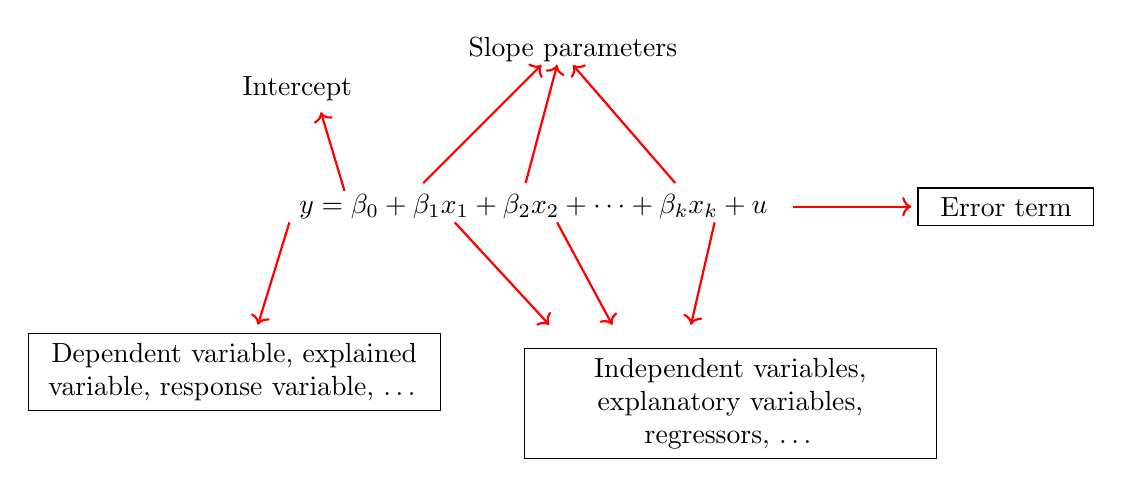
\begin{tikzpicture}

    % Equation
    \node at (0, 0) {\( y = \beta_0 + \beta_1 x_1 + \beta_2 x_2 + \dots + \beta_k x_k + u \)};

    % Annotation for y (Dependent variable)
    \node[draw, rectangle, text width=5cm, align=center] at (-3.8, -2.1) {Dependent variable, explained variable, response variable, \dots};
    \draw[->, red, thick] (-3.1,-0.2) -- (-3.5,-1.5);

    % Annotation for beta_0 (Intercept)
    \node[align=center] at (-3, 1.5) {Intercept};
    \draw[->, red, thick] (-2.4, 0.2) -- (-2.7, 1.2);

    % Annotation for all slope parameters (beta_1, beta_2, ..., beta_k)
    \node[align=center] at (0.5, 2) {Slope parameters};
    \draw[->, red, thick] (-1.4, 0.3) -- (0.1, 1.8);
    \draw[->, red, thick] (-0.1, 0.3) -- (0.3, 1.8);
    \draw[->, red, thick] (1.8, 0.3) -- (0.5, 1.8);

    % Annotation for all explanatory variables (x_1, x_2, ..., x_k)
    \node[draw, rectangle, text width=5cm, align=center] at (2.5, -2.5) {Independent variables,\\ explanatory variables,\\regressors, \dots};
    \draw[->, red, thick] (-1,-0.2) -- (0.2,-1.5);
    \draw[->, red, thick] (0.3,-0.2) -- (1.0,-1.5);
    \draw[->, red, thick] (2.3,-0.2) -- (2.0,-1.5);

    % Annotation for u (Error term)
    \node[draw, rectangle, text width=2cm, align=center] at (6, 0) {Error term};
    \draw[->, red, thick] (3.3, 0) -- (4.8,0);

\end{tikzpicture}




}

%%%%%%%%%%%%%%%%%%%%%%%%%%

\frame<beamer>{\frametitle{\textcolor{CUNEFOrange}{Motivation for multiple regression
}}


\begin{itemize}

\item Incorporate more explanatory factors into the model
\item Explicitly hold other factors fixed while examining the effects
of a particular independent variable on the dependent variable.
\item Allow for more flexible functional forms
\item \textbf{Example: Wage equation}\medskip


\tikzset{every picture/.style={line width=0.75pt}} %set default line width to 0.75pt        

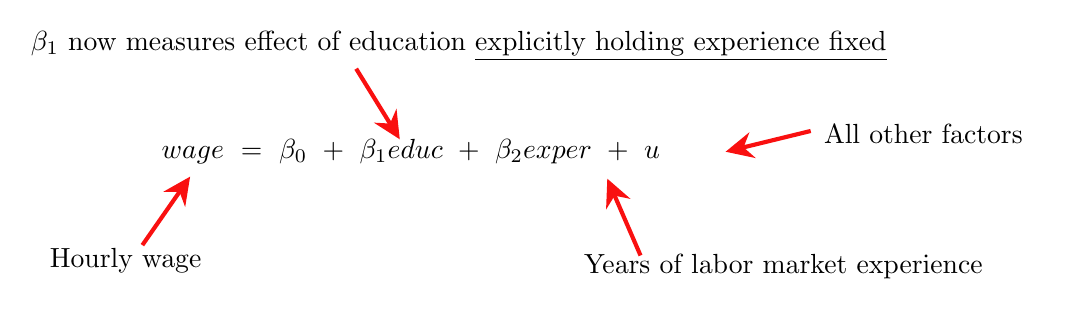
\begin{tikzpicture}[x=0.75pt,y=0.75pt,yscale=-1,xscale=1]
%uncomment if require: \path (0,300); %set diagram left start at 0, and has height of 300

%Straight Lines [id:da2117384336082615] 
\draw [color={rgb, 255:red, 249; green, 16; blue, 16 }  ,draw opacity=1 ][line width=1.5]    (114,200.5) -- (122.39,188.47) -- (134.71,170.78) ;
\draw [shift={(137,167.5)}, rotate = 124.88] [fill={rgb, 255:red, 249; green, 16; blue, 16 }  ,fill opacity=1 ][line width=0.08]  [draw opacity=0] (13.4,-6.43) -- (0,0) -- (13.4,6.44) -- (8.9,0) -- cycle    ;
%Straight Lines [id:da33077232559941905] 
\draw [color={rgb, 255:red, 249; green, 16; blue, 16 }  ,draw opacity=1 ][line width=1.5]    (217,115.5) -- (235.9,146.1) ;
\draw [shift={(238,149.5)}, rotate = 238.3] [fill={rgb, 255:red, 249; green, 16; blue, 16 }  ,fill opacity=1 ][line width=0.08]  [draw opacity=0] (13.4,-6.43) -- (0,0) -- (13.4,6.44) -- (8.9,0) -- cycle    ;
%Straight Lines [id:da6863882187517996] 
\draw [color={rgb, 255:red, 249; green, 16; blue, 16 }  ,draw opacity=1 ][line width=1.5]    (354,205.5) -- (339.59,172.17) ;
\draw [shift={(338,168.5)}, rotate = 66.61] [fill={rgb, 255:red, 249; green, 16; blue, 16 }  ,fill opacity=1 ][line width=0.08]  [draw opacity=0] (13.4,-6.43) -- (0,0) -- (13.4,6.44) -- (8.9,0) -- cycle    ;
%Straight Lines [id:da5743083478701962] 
\draw [color={rgb, 255:red, 249; green, 16; blue, 16 }  ,draw opacity=1 ][line width=1.5]    (436,145.5) -- (398.89,154.55) ;
\draw [shift={(395,155.5)}, rotate = 346.29] [fill={rgb, 255:red, 249; green, 16; blue, 16 }  ,fill opacity=1 ][line width=0.08]  [draw opacity=0] (13.4,-6.43) -- (0,0) -- (13.4,6.44) -- (8.9,0) -- cycle    ;

% Text Node
\draw (122,148.4) node [anchor=north west][inner sep=0.75pt]    {$wage\ =\ \beta _{0} \ +\ \beta _{1} educ\ +\ \beta _{2} exper\ +\ u$};
% Text Node
\draw (112.5,207.75) node   [align=left] {\begin{minipage}[lt]{64.6pt}\setlength\topsep{0pt}
Hourly wage
\end{minipage}};
% Text Node
\draw (59,96) node [anchor=north west][inner sep=0.75pt]   [align=left] {$\beta_1$ now measures effect of education \underline{explicitly holding experience fixed}};
% Text Node
\draw (431.5,210.75) node   [align=left] {\begin{minipage}[lt]{157.08pt}\setlength\topsep{0pt}
Years of labor market experience
\end{minipage}};
% Text Node
\draw (495,146.75) node   [align=left] {\begin{minipage}[lt]{78.88pt}\setlength\topsep{0pt}
All other factors
\end{minipage}};


\end{tikzpicture}
\end{itemize}

}

%%%%%%%%%%%%%%%%%%%%%%%%%%

\frame<beamer>{\frametitle{\textcolor{CUNEFOrange}{Motivation for multiple regression}}


\begin{itemize}

\item Example: CEO salary, sales and CEO tenure\\
\begin{figure}
    \centering
    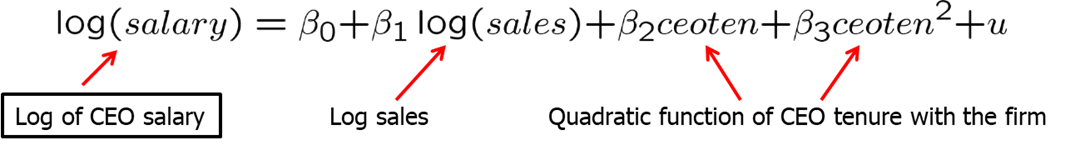
\includegraphics[width=0.9\linewidth]{figs/ceo_salary.png}
\end{figure}

\item Model assumes a quadratic relationship between CEO salary and his or her tenure with the firm
\[
\frac{\partial \log(\text{salary})}{\partial \text{ceoten}} = \beta_2 + 2\beta_3 \text{ceoten}
\]
The increase in salary due to additional years of tenure depends on how many years the CEO has already been with the firm. 

\item The model has to be linear in the parameters (not in the variables!).

\end{itemize}

}

%%%%%%%%%%%%%%%%%%%%%%%%%%
\section{OLS estimation in Multiple Regression}
\frame<beamer>{\frametitle{\textcolor{CUNEFOrange}{OLS estimation in Multiple Regression Analysis}}


\begin{itemize}

\item Random sample
$$
\left\{\left(x_{i 1}, x_{i 2}, \ldots, x_{i k}, y_i\right): \quad i=1, \ldots, n\right\}
$$

\item Regression residuals
$$
\widehat{u}_i=y_i-\widehat{\beta}_0-\widehat{\beta}_1 x_{i 1}-\widehat{\beta}_2 x_{i 2}-\ldots-\widehat{\beta}_k x_{i k}
$$

\item Minimize sum of squared residuals
$$
\min \text{SSR} = \min \sum_{i=1}^n \widehat{u}_i^2 \rightarrow \widehat{\beta}_0, \widehat{\beta}_1, \widehat{\beta}_2, \ldots, \widehat{\beta}_k
$$


\end{itemize}

}

%%%%%%%%%%%%%%%%%%%%%%%%%%

\frame<beamer>{\frametitle{\textcolor{CUNEFOrange}{Interpretation of the multiple regression model
}}


$$
\beta_j=\frac{\Delta y}{\Delta x_j} \longleftarrow \begin{aligned}
& \text { By how much does the dependent variable change if the } j \text {-th } \\
& \text { independent variable is increased by one unit, holding all } \\
& \text { other independent variables constant }
\end{aligned}
$$


\begin{itemize}
\item  The multiple linear regression model manages to hold the values of other explanatory variables fixed even if, in reality, they are correlated with the explanatory variable under consideration.
\item  ``Ceteris paribus'' interpretation
\item  It has still to be assumed that unobserved factors do not change if the explanatory variables are changed.

\end{itemize}

}

%%%%%%%%%%%%%%%%%%%%%%%%%%

\frame<beamer>{\frametitle{\textcolor{CUNEFOrange}{Interpretation of the multiple regression model}}


\begin{itemize}

\item Example: Determinants of college GPA
\begin{figure}
    \centering
    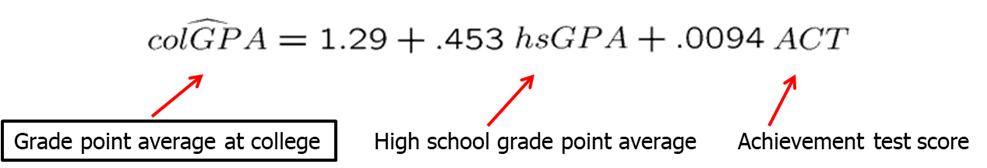
\includegraphics[width=0.8\linewidth]{figs/gpa.png}
\end{figure}

\item Interpretation
\begin{itemize}
    \item Holding ACT fixed, another point on high school grade point average is associated with another .453 points college grade point average
\item  Or: If we compare two students with the same ACT, but the hsGPA of student A is one point higher, we predict student A to have a colGPA that is .453 higher than that of student B
\item  Holding high school grade point average fixed, another 10 points on ACT are associated with less than one point on college GPA
\end{itemize}
\end{itemize}

}

%%%%%%%%%%%%%%%%%%%%%%%%%%
\section{Properties of OLS in multiple regression}
\frame<beamer>{\frametitle{\textcolor{CUNEFOrange}{Properties of OLS on any sample of data
}}


\begin{enumerate}
    \item Fitted (predicted) values 
$$
\widehat{y}_i=\widehat{\beta}_0+\widehat{\beta}_1 x_{i 1}+\widehat{\beta}_2 x_{i 2}+\ldots+\widehat{\beta}_k x_{i k}
$$

\item Residuals (deviations from the regression line)
$$
\widehat{u}_i=y_i-\widehat{y}_i
$$

    \item Deviations from regression line sum up to zero:    $$
\sum_{i=1}^n \widehat{u}_i=0
$$

\item Covariance between deviations and regressors is zero
$$
\sum_{i=1}^n x_i \widehat{u}_i=0
$$

\item Sample averages of $y$ and the regressors lie on regression line
$$
\bar{y}=\widehat{\beta}_0+\widehat{\beta}_1 \bar{x}_1+\ldots+\widehat{\beta}_k \bar{x}_k
$$

\end{enumerate}
}


%%%%%%%%%%%%%%%%%%%%%%%%%%
\section{Goodness-of-Fit}

\frame<beamer>{\frametitle{\textcolor{CUNEFOrange}{Goodness-of-Fit
}}


\begin{itemize}

\item Decomposition of total variation
$$
SST=SSE+SSR
$$

\item R-squared: $R^2 \equiv S S E / S S T=1-S S R / S S T$


\item Notice that R-squared can only increase if another explanatory variable is added to the regression

\item Alternative expression for $R$-squared
$$
R^2=\frac{\left(\sum_{i=1}^n\left(y_i-\bar{y}\right)\left(\widehat{y}_i-\overline{\widehat{y}}\right)\right)^2}{\left(\sum_{i=1}^n\left(y_i-\bar{y}\right)^2\right)\left(\sum_{i=1}^n\left(\widehat{y}_i-\overline{\hat{y}}\right)^2\right)}
$$
\textbf{R-squared is equal to the squared correlation coefficient between the actual and the predicted value of the dependent variable}

\end{itemize}

}

%%%%%%%%%%%%%%%%%%%%%%%%%%

\frame<beamer>{\frametitle{\textcolor{CUNEFOrange}{Goodness-of-Fit}}

\begin{itemize}
    \item The following regression model aims to explain the ROE in terms of several financial metrics:
\end{itemize}

\begin{align}
\widehat{\text{ROE}} = &0.153 - 0.075 \times \text{Leverage} + 0.032 \times \text{Asset Turnover} \nonumber\\
&- 0.014 \times \text{Operating Expenses} + 0.062 \times \text{Market Share}\nonumber\\
&R^2 = 0.0413\nonumber
\end{align}


\begin{itemize}
    \item Interpretation:
    \begin{itemize}
        \item If leverage increases by 1 unit, the predicted ROE decreases by 7.5 percentage points.
        \item If asset turnover increases by 1 unit, the predicted ROE increases by 3.2 percentage points.
        \item Higher operating expenses decrease ROE, while greater market share improves ROE.
    \end{itemize}
\end{itemize}

}

%%%%%%%%%%%%%%%%%%%%%%%%%%

\frame<beamer>{\frametitle{\textcolor{CUNEFOrange}{Goodness-of-Fit}}


\begin{itemize}
    \item An additional explanatory variable is added: Dividend Payout Ratio
\end{itemize}

\begin{align}
\widehat{\text{ROE}} = &0.153 - 0.075 \times \text{Leverage} + 0.032 \times \text{Asset Turnover} \nonumber\\
&- 0.014 \times \text{Operating Expenses} + 0.062 \times \text{Market Share}\nonumber \\
&+ \alert{0.025 \times \text{Dividend Payout Ratio}}\nonumber\\
& R^2 = 0.0422
\end{align}

\begin{itemize}
    \item Interpretation:
    \begin{itemize}
        \item The dividend payout ratio has a small positive effect on ROE.
        \item The additional explanatory power of the model is limited, as R-squared increases only slightly.
    \end{itemize}
\end{itemize}

}

%%%%%%%%%%%%%%%%%%%%%%%%%%
\section{Assumptions for the multiple regression model}
\frame<beamer>{\frametitle{\textcolor{CUNEFOrange}{Standard assumptions for the multiple regression model}}

\begin{itemize}
    \item \textbf{Assumption MLR.1} (Linear in parameters): In the population, the relationship between $y$ and the explanatory variables is linear
    $$
y=\beta_0+\beta_1 x_1+\beta_2 x_2+\ldots+\beta_k x_k+u
$$

\item \textbf{Assumption MLR.2} (Random sampling): The data is a random sample drawn from the population
$$
\left\{\left(x_{i 1}, x_{i 2}, \ldots, x_{i k}, y_i\right): i=1, \ldots, n\right\}
$$
Each data point therefore follows the population equation
$$
y_i=\beta_0+\beta_1 x_{i 1}+\beta_2 x_{i 2}+\ldots+\beta_k x_{i k}+u_i
$$



\end{itemize}




}

%%%%%%%%%%%%%%%%%%%%%%%%%%

\frame<beamer>{\frametitle{\textcolor{CUNEFOrange}{Standard assumptions for the multiple regression model}}


\begin{itemize}

\item \textbf{Assumption MLR.3} (No perfect collinearity): In the sample (and therefore in the population), none of the independent variables is constant and there are no exact linear relationships among the independent variables.
\medskip

\item Remarks on MLR.3
\begin{itemize}
    \item The assumption only rules out perfect collinearity/correlation between explanatory variables; imperfect correlation is allowed.

    \item If an explanatory variable is a perfect linear combination of other explanatory variables it is superfluous and may be eliminated.

    \item Constant variables are also ruled out (collinear with intercept).

\end{itemize}


\end{itemize}

}

%%%%%%%%%%%%%%%%%%%%%%%%%%

\frame<beamer>{\frametitle{\textcolor{CUNEFOrange}{Standard assumptions for the multiple regression model}}


\begin{itemize}

\item Example for perfect collinearity: small sample
$$
\text { avgscore }=\beta_0+\beta_1 \text { expend }+\beta_2 \text { avginc }+u
$$
In a small sample, avginc may accidentally be an exact multiple of expend; it will not be possible to disentangle their separate effects because there is exact covariation

\item Example for perfect collinearity: relationships between regressors
$$
\operatorname{vote} A=\beta_0+\beta_1 \text { share } A+\beta_2 \text { share } B+u
$$
Either shareA or shareB will have to be dropped from the regression because there is an exact linear relationship between them: share $A$ + share $B=1$
\end{itemize}

}

%%%%%%%%%%%%%%%%%%%%%%%%%%

\frame<beamer>{\frametitle{\textcolor{CUNEFOrange}{Standard assumptions for the multiple regression model}}


\begin{itemize}

\item \textbf{Assumption MLR.4} (Zero conditional mean): The value of the explanatory variables must contain no information about the mean of the unobserved factors
$$
E\left(u_i \mid x_{i 1}, x_{i 2}, \ldots, x_{i k}\right)=0
$$
In a multiple regression model, the zero conditional mean assumption is much more likely to hold because fewer things end up in the error.


\end{itemize}

}

%%%%%%%%%%%%%%%%%%%%%%%%%%

\frame<beamer>{\frametitle{\textcolor{CUNEFOrange}{Including irrelevant variables in a regression model
}}


\begin{itemize}

\item Consider the multiple regression model:
$$
y=\beta_0+\beta_1 x_1+\beta_2 x_2+\beta_3x_3+u
$$
Suppose that, in the population, variable $x_3$ is irrelevant such that $\beta_3=0$. 

\item Since OLS estimates are unbiased,
$$
E\left(\widehat{\beta}_3\right)=\beta_3=0
$$
There is no problem in including irrelevant variables.

\item \alert{Warning:} However, including irrevelant variables may increase sampling variance.
\end{itemize}

}

%%%%%%%%%%%%%%%%%%%%%%%%%%

\frame<beamer>{\frametitle{\textcolor{CUNEFOrange}{Omitting relevant variables: the simple case
}}


\begin{itemize}

\item Suppose the true model contains $x_1$ and $x_2$:
$$
y=\beta_0+\beta_1 x_1+\beta_2 x_2+u
$$

\item Suppose that, in the estimated model, $x_2$ is ommited:
$$
\tilde{y}=\tilde{\beta}_0+\tilde{\beta}_1 x_1+\tilde{u}
$$
This leads to a \alert{ommited variable bias}.




\end{itemize}

}

%%%%%%%%%%%%%%%%%%%%%%%%%%

\frame<beamer>{\frametitle{\textcolor{CUNEFOrange}{Omitting relevant variables: the simple case}}


\begin{itemize}

\item  If $x_1$ and $x_2$ are correlated, assume a linear regression relationship between them:
$$
x_2=\delta_0+\delta_1 x_1+v
$$

\item Substituting in the equation of the true model:
\begin{align}
y=&\beta_0+\beta_1 x_1+\beta_2\left(\delta_0+\delta_1 x_1+v\right)+u \nonumber\\
=&\underbrace{\left(\beta_0 + \beta_2 \delta_0\right)}_{\text{Intercept}} 
+ \underbrace{\left(\beta_1 + \beta_2 \delta_1\right)}_{\text{Coefficient of } x_1} x_1 
+ \underbrace{\left(\beta_2 v + u\right)}_{\text{Error term}}\nonumber
\end{align}

\item If $y$ is only regressed on $x_1$, and $x_1$ is correlated with $x_2$, \alert{all coefficients in will be biased}.

\end{itemize}

}

%%%%%%%%%%%%%%%%%%%%%%%%%%

\frame<beamer>{\frametitle{\textcolor{CUNEFOrange}{Omitting relevant variables: the simple case}}


\begin{itemize}

\item Example: Omitting ability in a wage equation
\begin{figure}
    \centering
    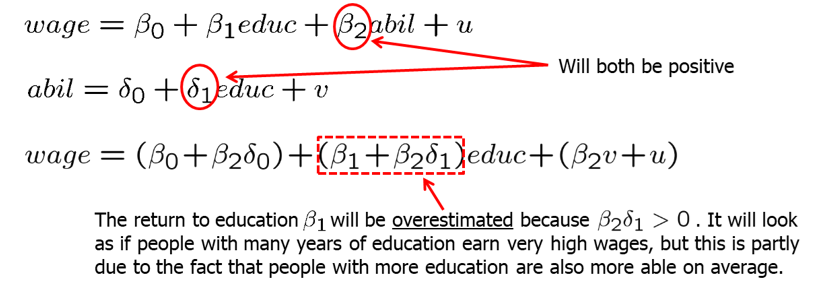
\includegraphics[width=1\linewidth]{figs/omitted_wage.png}
\end{figure}

\end{itemize}

}

%%%%%%%%%%%%%%%%%%%%%%%%%%

\frame<beamer>{\frametitle{\textcolor{CUNEFOrange}{Standard assumptions for the multiple regression model (cont.)}}


\begin{itemize}

\item \textbf{Assumption MLR.5} (Homoskedasticity): The value of the explanatory variables must contain no information about the variance of the unobserved factors
$$
\operatorname{Var}\left(u_i \mid x_{i 1}, x_{i 2}, \ldots, x_{i k}\right)=\sigma^2
$$

\item Example: Wage equation
$$
\operatorname{Var}\left(u_i \mid \text { educ }_i, \text { exper }_i, \text { tenur }_i\right)=\sigma^2
$$
This assumption may also be hard to justify in many cases
\end{itemize}

}

%%%%%%%%%%%%%%%%%%%%%%%%%%
\section{Sampling variances of the OLS estimators}
\frame<beamer>{\frametitle{\textcolor{CUNEFOrange}{Sampling variances of the OLS slope estimators}}


\begin{itemize}

\item Theorem: Under assumptions MLR.1 – MLR.5:
\begin{figure}
    \centering
    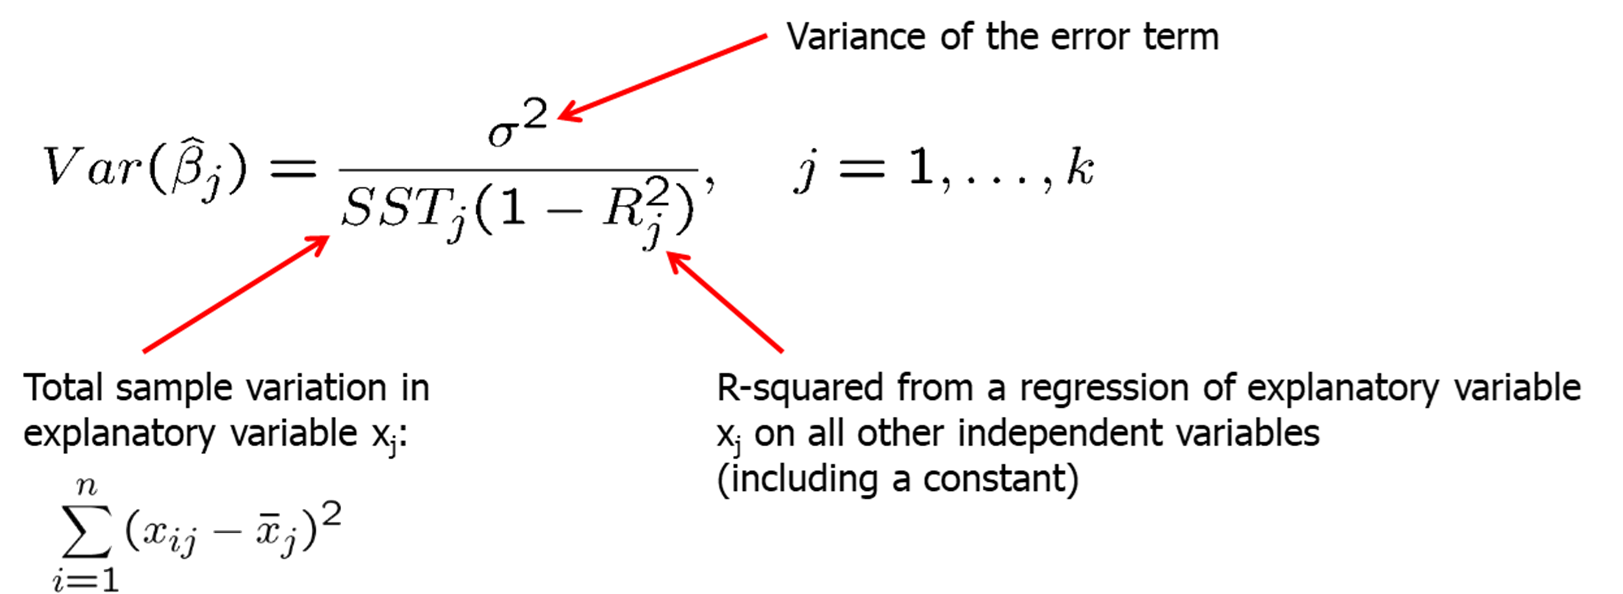
\includegraphics[width=1\linewidth]{figs/var.png}
\end{figure}

\end{itemize}

}

%%%%%%%%%%%%%%%%%%%%%%%%%%

\frame<beamer>{\frametitle{\textcolor{CUNEFOrange}{Components of OLS Variances}}



    \begin{enumerate}
        \item \textbf{The error variance}
        \begin{itemize}
            \item A high error variance increases the sampling variance because there is more "noise" in the equation.
            \item A large error variance doesn't necessarily make estimates imprecise.
            \item The error variance does not decrease with sample size.
        \end{itemize}
        \item \textbf{The total sample variation in the explanatory variable}
        \begin{itemize}
            \item More sample variation leads to more precise estimates.
            \item Total sample variation automatically increases with the sample size.
            \item Increasing the sample size is thus a way to get more precise estimates.
        \end{itemize}
        \item \textbf{Linear relationships among the independent variables}
        \begin{itemize}
            \item Regress $\mathrm{x}_{\mathrm{j}}$ on all other independent variables (including constant).
            \item The R-squared of this regression will be higher when $x_i$ can be better explained by the other independent variables.
            \item The sampling variance of the slope estimator for $\mathrm{x}_{\mathrm{i}}$ will be higher when $\mathrm{x}_{\mathrm{i}}$ can be better explained by the other independent variables.
            \item Under perfect multicollinearity, the variance of the slope estimator will approach infinity.
        \end{itemize}
    \end{enumerate}


}

%%%%%%%%%%%%%%%%%%%%%%%%%%

\frame<beamer>{\frametitle{\textcolor{CUNEFOrange}{The multicollinearity problem}}


\begin{itemize}

\item When two explanatory variables are correlated (colinear), it is difficult to \textbf{disentangle} the effect of each variable 

\item \textbf{Example: Debt and Interest Expense}.   Consider the following regression model:
    \[
    \text{ROA} = \beta_0 + \beta_1 \times \text{Debt} + \beta_2 \times \text{Interest Expense} + \epsilon
    \]

 \item In this case, Debt and Interest Expense are likely to be highly correlated.
        \item As companies take on more debt, their interest expense generally increases, making it difficult to separate their individual effects on ROA.
        
            \item Difficulty in interpreting whether changes in ROA are driven more by Debt or by Interest Expense.

\item We might consider removing one of the two variables from the equation (but this may lead to omitted variable bias).
    \end{itemize}


}


%%%%%%%%%%%%%%%%%%%%%%%%%%

\frame<beamer>{\frametitle{\textcolor{CUNEFOrange}{The multicollinearity problem}}


\begin{itemize}

\item What is the effect of multicollinearity on OLS estimates?

\item Only the sampling variance of the variables involved in multicollinearity will be inflated; the estimates of other effects may be very precise.

\item Note that multicollinearity is not a violation of MLR.3 in the strict sense.

\item Multicollinearity may be detected through ``\textbf{variance inflation factors}''
$$
\text{VIF}_j=1 /\left(1-R_j^2\right)
$$
As an (arbitrary) rule of thumb, the variance inflation factor should not be larger than 10

\end{itemize}


}

%%%%%%%%%%%%%%%%%%%%%%%%%%

\frame<beamer>{\frametitle{\textcolor{CUNEFOrange}{
Variances in misspecified models
}}


\begin{itemize}

\item The choice of whether to include a particular variable in a regression can be made by analyzing the \textbf{tradeoff between bias and variance}.

\item Consider the following population and estimated models:

\item True population model:
$$
y=\beta_0+\beta_1 x_1+\beta_2 x_2+u
$$

\item Estimated model 1:
$$
\widehat{y}=\widehat{\beta}_0+\widehat{\beta}_1 x_1+\widehat{\beta}_2 x_2
$$

\item Estimated model 2:
$$
\tilde{y}=\tilde{\beta}_0+\tilde{\beta}_1 x_1
$$
\end{itemize}


}

%%%%%%%%%%%%%%%%%%%%%%%%%%

\frame<beamer>{\frametitle{\textcolor{CUNEFOrange}{
Variances in misspecified models
}}


\begin{itemize}

\item Estimated model 1:
$$
\widehat{y}=\widehat{\beta}_0+\widehat{\beta}_1 x_1+\widehat{\beta}_2 x_2
$$
$$
\operatorname{Var}\left(\widehat{\beta}_1\right)=\sigma^2 /\left[S S T_1\left(1-R_1^2\right)\right]
$$

\item Estimated model 2:
$$
\tilde{y}=\tilde{\beta}_0+\tilde{\beta}_1 x_1
$$
$$
\operatorname{Var}\left(\widetilde{\beta}_1\right)=\sigma^2 / S S T_1
$$

\item Which one is smaller, $\operatorname{Var}\left(\widehat{\beta}_1\right)$ or $\operatorname{Var}\left(\widetilde{\beta}_1\right)$?
\begin{itemize}
    \item Conditional on $x_1$ and $x_2$, the variance in model 2 is always smaller than that in model 1.
    \item However, model 2 will lead to biased estimates (due to omitted variable bias)! 
    \item  We can evaluate the \textbf{trade-off between bias and variance}.
\end{itemize}

\end{itemize}


}



%%%%%%%%%%%%%%%%%%%%%%%%%%

\frame<beamer>{\frametitle{\textcolor{CUNEFOrange}{
Estimating the error variance
}}


\begin{itemize}

\item An unbiased estimate of the error variance can be obtained by subtracting the number of estimated regression coefficients from the number of observations.
$$
\widehat{\sigma}^2=\left(\sum_{i=1}^n \widehat{u}_i^2\right) /[n-k-1]
$$

\item The number of observations minus the number of estimated parameters is also called the degrees of freedom. 

\item Theorem: Under MLR. 1 -- MLR.5,
$$
E\left(\hat{\sigma}^2\right)=\sigma^2
$$

\end{itemize}


}

%%%%%%%%%%%%%%%%%%%%%%%%%%

\frame<beamer>{\frametitle{\textcolor{CUNEFOrange}{
Estimation of the sampling variances of the OLS estimators
}}


\begin{itemize}

\item The estimated sampling variation (or standard error) of the estimated $\beta_j$ is given by 
$$
se\left(\widehat{\beta}_j\right)=\sqrt{\widehat{\operatorname{Var}}\left(\widehat{\beta}_j\right)}=\sqrt{\frac{\widehat{\sigma}^2}{SST_j\left(1-R_j^2\right)}}
$$

\item Note that in the above formula we use the unbiased estimate of the error variance,  $\widehat{\sigma}^2$.

\item Moreover, this formula is only valid under assumptions   MLR.1-MLR.5 (in particular, there has to be homoskedasticity).

\end{itemize}


}


%%%%%%%%%%%%%%%%%%%%%%%%%%

\frame<beamer>{\frametitle{\textcolor{CUNEFOrange}{
Efficiency of OLS: The Gauss-Markov Theorem
}}


\begin{itemize}

\item  Under assumptions MLR. 1 - MLR.5, OLS is unbiased
\item However, under these assumptions there may be many other estimators that are unbiased.
\item Which one is the unbiased estimator with the smallest variance?
\item In order to answer this question one usually limits oneself to linear estimators, i.e. estimators linear in the dependent variable.

$$
\tilde{\beta}_j=\sum_{i=1}^n w_{i j} y_i \longleftarrow \begin{aligned}
& \text { May be an arbitrary function of the sample values } \\
& \text { of all the explanatory variables; the OLS estimator } \\
& \text { can be shown to be of this form }
\end{aligned}
$$


\end{itemize}


}

%%%%%%%%%%%%%%%%%%%%%%%%%%

\frame<beamer>{\frametitle{\textcolor{CUNEFOrange}{
Efficiency of OLS: The Gauss-Markov Theorem
}}


\begin{itemize}

\item Under assumptions MLR. 1 - MLR.5, the OLS estimators are the best linear unbiased estimators (BLUEs) of the regression coefficients, i.e.
$$
\operatorname{Var}\left(\widehat{\beta}_j\right) \leq \operatorname{Var}\left(\widetilde{\beta}_j\right) \quad j=0,1, \ldots, k
$$
for all $\tilde{\beta}_j=\sum_{i=1}^n w_{i j} y_i$ for which $E\left(\widetilde{\beta}_j\right)=\beta_j, j=0, \ldots, k$.

\item OLS is only the best estimator if MLR. 1 - MLR. 5 hold; if there is heteroskedasticity for example, there are better estimators.

\end{itemize}


}

%%%%%%%%%%%%%%%%%%%%%
% Back Page
%%%%%%%%%%%%%%%%%%%%
\NoLogoFootline
{\usebackgroundtemplate{%

\includegraphics[width=\paperwidth,height=\paperheight]{figs/back_page.png}}
\slide{}{}}







\end{document}